\documentclass{article}
    % General document formatting
    \usepackage[margin=0.7in]{geometry}
    \usepackage[parfill]{parskip}
    \usepackage[utf8]{inputenc}
    
    % Related to math
    \usepackage{amsmath,amssymb,amsfonts,amsthm}
\usepackage{graphicx}
%\usepackage{subfig}
%\usepackage{subfigure}
\usepackage{caption}
\usepackage{subcaption}
\usepackage{listings}
\usepackage[percent]{overpic}
\usepackage{xcolor,varwidth}

\definecolor{green}{HTML}{008000}
\definecolor{blue}{HTML}{0000ff}
\definecolor{yellow}{HTML}{bfbf00}
\definecolor{cyan}{HTML}{00bfbf}
\definecolor{magenta}{HTML}{bf00bf}
\definecolor{lime}{HTML}{00FF00}
\definecolor{purple}{HTML}{9933FF}
\definecolor{pink}{HTML}{FF66FF}
\definecolor{grey}{HTML}{d3d3d3}

\usepackage{titling}
%\usepackage{lipsum}

\usepackage{titlesec}

\titleformat*{\section}{\large\bfseries}
\titleformat*{\subsection}{\large\bfseries}
%\titleformat*{\subsubsection}{\large\bfseries}
%\titleformat*{\paragraph}{\large\bfseries}
%\titleformat*{\subparagraph}{\large\bfseries}
\titlespacing\section{0pt}{6pt plus 4pt minus 2pt}{0pt plus 2pt minus 2pt}
\titlespacing\subsection{0pt}{6pt plus 4pt minus 2pt}{0pt plus 2pt minus 2pt}
\titlespacing\subsubsection{0pt}{12pt plus 4pt minus 2pt}{0pt plus 2pt minus 2pt}

\pretitle{\begin{center}\large\bfseries}
\posttitle{\par\end{center}\vskip 0.01em}
\preauthor{\begin{center}\Large\ttfamily}
\postauthor{\end{center}}
\predate{\par\normalsize\centering}
\postdate{\par}

\title{Population Genetic Analyses of Genomic Data 1}
%\date{\today}

\begin{document}

%\maketitle

\begin{center}
\textbf{\Large{\centering{Cancer Evolution 1}}}\\
\textit{USN: 303039534}
\end{center}
%\normalsize{   }
%~\\

\section{}

Figures 1b, 1c and 1d  were generated using python and matplotlib. Figure 1a was generated using the python networkx module and visualized using cytoscape. All code is given in the appendix, and additional annotations were added using the \LaTeX \, overpic package.\\\\


\begin{figure}[h]
	\centering
	\begin{subfigure}[t]{0.243\linewidth}
		\centering
		\begin{overpic}[width=1.0\textwidth, trim={48 4 48 0}, clip=true]{graph.png}
			\put(14,103){\rotatebox{0}{\color{black}\normalsize Clonal evolution }}

			\put(38,95){\color{black} \large \textit{\textbf{0}}}
			\put(38,78){\color{black} \large \textit{\textbf{A}}}
			\put(38,58){\color{black} \large \textit{\textbf{AB}}}
			\put(38,39){\color{black} \large \textit{\textbf{ABC}}}

			\put(46,27){\color{black} \large \textit{\textbf{ABCD}}}
			\put(20,3){\color{black} \large \textit{\textbf{ABCDH}}}
			\put(49,3){\color{black} \large \textit{\textbf{ABCDG}}}

			\put(-1.5,27){\color{black} \large \textit{\textbf{ABCE}}}
			\put(-7.5,3){\color{black} \large \textit{\textbf{ABCEF}}}
		\end{overpic}

		\subcaption{}
		\label{a}
	\end{subfigure}%
	\hspace{0.15\linewidth}
	\begin{subfigure}[t]{0.58\linewidth}
		\centering
		\begin{overpic}[width=1.0\textwidth, trim={0 0 0 40}, clip=true]{squares.png}

			
			%%%%%horizontal text

			\put(-9,5){\color{black}\small Cellular fraction}
			\put(-13.3,2){\color{black}\small Cancer cell fraction}

			\put(13,11.3){\color{black}\rule{0.738\textwidth}{1pt}}
			\put(16,8.5){\color{black}\small$A$}
			\put(15.8,5){\color{black}\small80}
			\put(15.8,2){\color{black}\small100}

			\put(21.5,11.3){\color{white}\rule{0.013\textwidth}{1pt}}
			\put(31,8){\color{black}\small$B$}
			\put(30.8,5){\color{black}\small60}
			\put(30.8,2){\color{black}\small75}

			\put(41.6,11.3){\color{white}\rule{0.013\textwidth}{1pt}}
			\put(44,8){\color{black}\small$C$}
			\put(43.8,5){\color{black}\small40}
			\put(43.8,2){\color{black}\small50}

			\put(47.5,11.3){\color{white}\rule{0.013\textwidth}{1pt}}
			\put(52,8){\color{black}\small$D$}
			\put(51.8,5){\color{black}\small24}
			\put(51.8,2){\color{black}\small30}

			\put(58,11.3){\color{white}\rule{0.013\textwidth}{1pt}}
			\put(62,8){\color{black}\small$E$}
			\put(61.8,5){\color{black}\small16}
			\put(61.8,2){\color{black}\small20}

			\put(68.9,11.3){\color{white}\rule{0.013\textwidth}{1pt}}
			\put(69.3,8){\color{black}\small$F$}
			\put(69.1,5){\color{black}\small12}
			\put(69.1,2){\color{black}\small15}

			\put(71.9,11.3){\color{white}\rule{0.013\textwidth}{1pt}}
			\put(75,8){\color{black}\small$G$}
			\put(74.8,5){\color{black}\small12}
			\put(74.8,2){\color{black}\small15}

			\put(80.5,11.3){\color{white}\rule{0.013\textwidth}{1pt}}
			\put(83,8){\color{black}\small$H$}
			\put(82.8,5){\color{black}\small12}
			\put(82.8,2){\color{black}\small15}
			%\put(0,10){\color{black}\rule{1pt}{30pt}}


			%%%%left side

			\put(9.5,33){\rotatebox{90}{\color{black}\large Cells}}

			\put(8,13.2){\rotatebox{90}{\color{black}\rule{0.477\textwidth}{1pt}}}

			\put(8,18.5){\rotatebox{90}{\color{white}\rule{0.013\textwidth}{1pt}}}
			\put(-5.7,14.5){\rotatebox{0}{\color{black}\small \textbf{\textit{ABCDG}} }}

			\put(8,24){\rotatebox{90}{\color{white}\rule{0.013\textwidth}{1pt}}}
			\put(-5.7,20.5){\rotatebox{0}{\color{black}\small \textbf{\textit{ABCDH}} }}

			\put(8,29.4){\rotatebox{90}{\color{white}\rule{0.013\textwidth}{1pt}}}
			\put(-5.7,26){\rotatebox{0}{\color{black}\small \textbf{\textit{ABCEF}} }}

			\put(8,32.2){\rotatebox{90}{\color{white}\rule{0.013\textwidth}{1pt}}}
			\put(-5.7,30.3){\rotatebox{0}{\color{black}\small \textbf{\textit{ABCE}} }}

			\put(8,41.6){\rotatebox{90}{\color{white}\rule{0.013\textwidth}{1pt}}}
			\put(-5.7,36.5){\rotatebox{0}{\color{black}\small \textbf{\textit{AB}} }}
			

			\put(8,50.8){\rotatebox{90}{\color{white}\rule{0.013\textwidth}{1pt}}}
			\put(-5.7,45.5){\rotatebox{0}{\color{black}\small \textbf{\textit{A}} }}

			\put(-5.7,55.5){\rotatebox{0}{\color{black}\small \textbf{\textit{0}} }}

			\put(-10,31){\rotatebox{90}{\color{black}\large Clones}}


			%%%right side

			\put(94,33){\rotatebox{0}{\color{black}\Large $\bf{\pi}$}}



			\put(87.8,13.2){\rotatebox{90}{\color{black}\rule{0.477\textwidth}{1pt}}}
			\put(89.5,17.2){\rotatebox{-90}{\color{black} 12} }

			\put(87.8,18.5){\rotatebox{90}{\color{white}\rule{0.013\textwidth}{1pt}}}
			\put(89.5,23.5){\rotatebox{-90}{\color{black} 12} }

			\put(87.8,24){\rotatebox{90}{\color{white}\rule{0.013\textwidth}{1pt}}}
			\put(89.5,29){\rotatebox{-90}{\color{black} 12} }

			\put(87.8,29.4){\rotatebox{90}{\color{white}\rule{0.013\textwidth}{1pt}}}
			\put(89.5,32.1){\rotatebox{-90}{\color{black} 4} }

			\put(87.8,32.2){\rotatebox{90}{\color{white}\rule{0.013\textwidth}{1pt}}}
			\put(89.5,39){\rotatebox{-90}{\color{black} 20} }

			\put(87.8,41.6){\rotatebox{90}{\color{white}\rule{0.013\textwidth}{1pt}}}
			\put(89.5,48.4){\rotatebox{-90}{\color{black} 20} }

			\put(87.8,50.8){\rotatebox{90}{\color{white}\rule{0.013\textwidth}{1pt}}}
			\put(89.5,57.6){\rotatebox{-90}{\color{black} 20} }


			%%%%%top

			\put(14,62){\rotatebox{0}{\color{black}\small 1 }}
			\put(84,62){\rotatebox{0}{\color{black}\small L }}
			\put(49,62){\rotatebox{0}{\color{black}\small ... }}

			\put(14,65){\rotatebox{0}{\color{black}\normalsize Genomic loci }}

			%\put(30,60){\colorbox{black}{ \parbox{0.1\linewidth} }{} }
			\put(36,65){\color{grey}\rule{0.016\textwidth}{5.8pt}}
			\put(38,65){\rotatebox{0}{\color{black}\tiny normal genotype }}


			\put(56,65){\color{green}\rule{0.016\textwidth}{5.8pt}}
			\put(58,65){\color{blue}\rule{0.016\textwidth}{5.8pt}}
			\put(60,65){\color{yellow}\rule{0.016\textwidth}{5.8pt}}
			\put(62,65){\color{cyan}\rule{0.016\textwidth}{5.8pt}}
			\put(64,65){\color{magenta}\rule{0.016\textwidth}{5.8pt}}
			\put(66,65){\color{lime}\rule{0.016\textwidth}{5.8pt}}
			\put(68,65){\color{purple}\rule{0.016\textwidth}{5.8pt}}
			\put(70,65){\color{pink}\rule{0.016\textwidth}{5.8pt}}

			\put(72,65){\rotatebox{0}{\color{black}\tiny mutations }}
			
		\end{overpic}

		%\centering
		%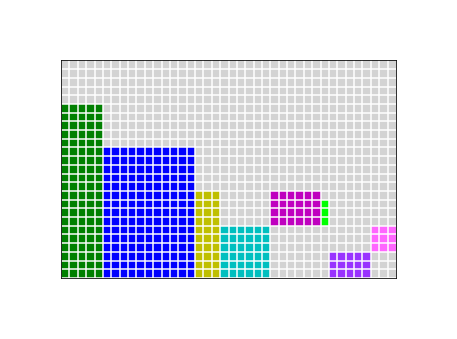
\includegraphics[width = 1.0\linewidth, trim={0 0 0 0}, clip=true]{squares.png}
		\caption{}
		\label{b}
	\end{subfigure}

	\par\bigskip

	%\vspace{0.15\linewidth}
	\begin{subfigure}[t]{0.35\linewidth}
		\centering
		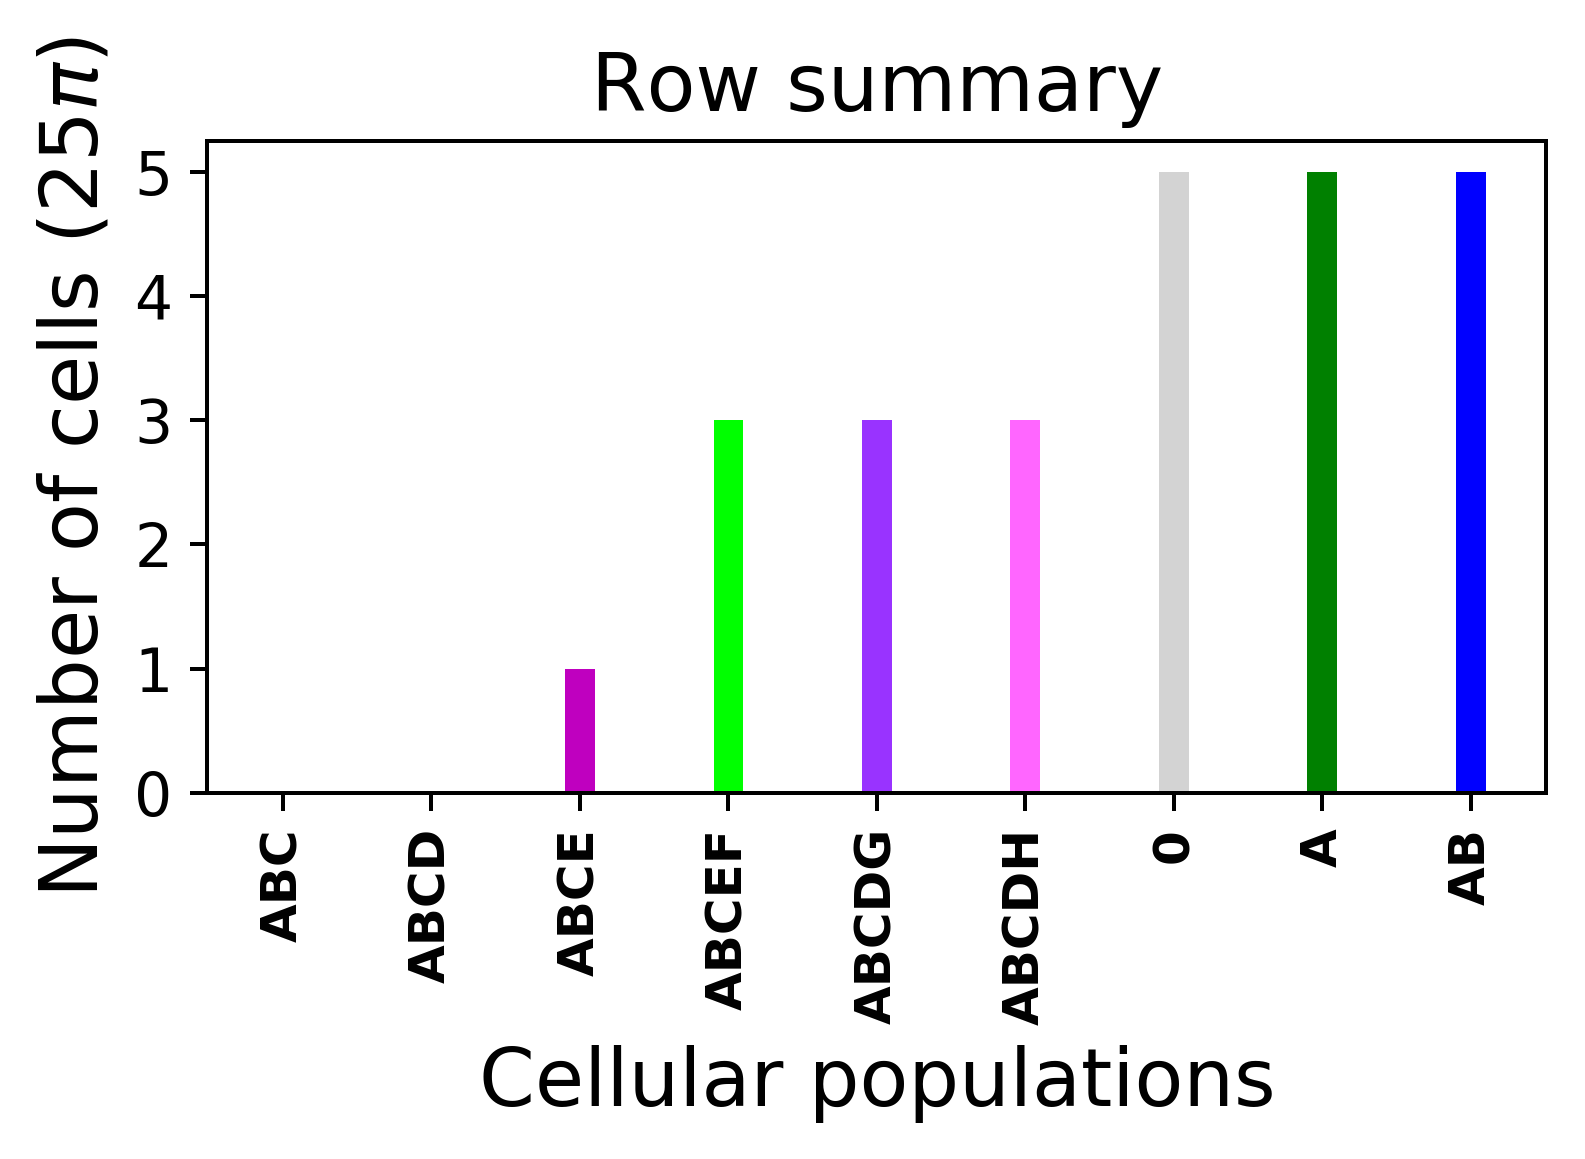
\includegraphics[width = 1.0\linewidth, trim={0 0 0 0}, clip=true]{rows.png}
		\caption{}
		\label{c}
	\end{subfigure}
	\hspace{0.1\linewidth}
	\begin{subfigure}[t]{0.35\linewidth}
		\centering
		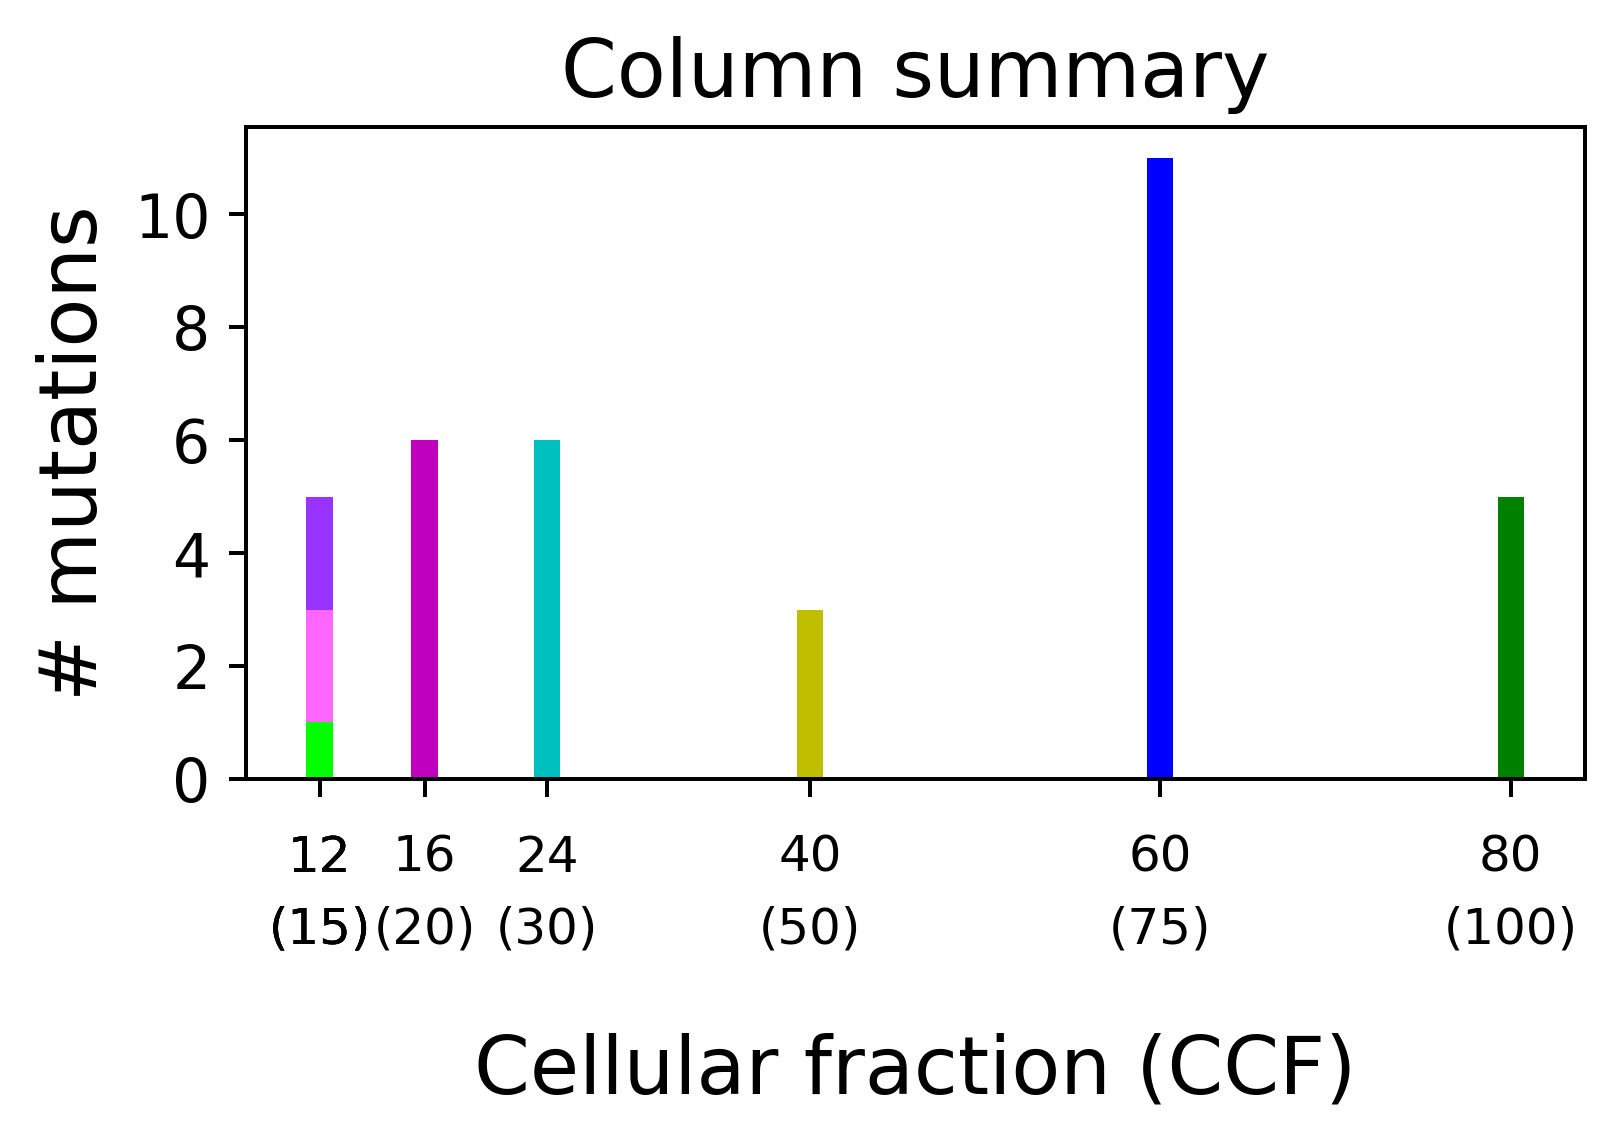
\includegraphics[width = 1.0\linewidth, trim={0 0 0 0}, clip=true]{cols.png}
		\caption{}
		\label{d}
	\end{subfigure}

\caption{
\textbf{(a)} Graph illustrating the evolution of the tumor. In constructing the graph, it has been assumed that no set of mutations has developed twice independently. Nodes represent clones and an edge between two nodes indicates that the daughter node has been derived from the parent node. Edges are labelled with the set of mutations giving rise to a particular clone, with labels A-H referring to the corresponding labels in figure (b). Nodes are labelled with their clonal frequency in percent and their genotype, again with reference to (b). \textbf{(b)} x-axis corresponds to 40 genetic loci of interest which have been used for the analysis. y-axis corresponds to 25 cells analyzed. Each letter A-H corresponds to a set of mutations at the corresponding loci. Colors refer to a set of cells having a given set of mutations. The genotype of any cell can thus be inferred by considering the set of colored squares for that particular row of the matrix. \textbf{(c)} Histogram showing the number of cells with each genotype from (a); the column heights sum to 25. \textbf{(d)} Histogram showing the number of loci mutated for a given transition in graph (a). x-axis represents the cellular fraction containing each particular set of mutations. Note that mutations F, G and H all have cellular fractions of 12\% and have been overlayed rather than stacked.
}
\end{figure}

\newpage



\setcounter{section}{2}

\subsection{}

In \textbf{figure 1a}, each node represents a single clone. For this purpose, we define a clone as a set of cells with the same mutation pattern at our 40 loci of interests (figure 1b). There is likely to be additional genetic variability at other loci within each clone, but we ignore this variability for the present purpose. The color of a node specifies the mutation pattern of the clone with reference to figure 1b. The colour corresponds to the last set of mutations that was aquired in a given clone; e.g. clone '\textit{AB}' has both mutations 'A' and mutations 'B' but is coloured blue as mutations 'B' were aquired on a background of 'A'. The label next to the node specifies the full genotype of the corresponding clone with reference to figure 1b.

In inferring the phylogenetic relationship between clones,  we assume that the same set of mutations has not developed multiple times independently and that no mutations have been reversed. This implies that a population of cells \{K\} with two sets of mutations \{X\} and \{Y\} must be descendants of a population of cells \{L\} that have mutations \{X\} but not \{Y\}. This allows us to construct an unambiguous phylogenetic tree from the single cell data in figure 1b.

The number on each node specifies the clonal frequency $\pi_k = \dfrac{N_k}{\sum_l{N_l}}$ represented by that particular clone where $N_k$ is the number of cells with genotype k. The clonal frequency is also represented by the size of the node. Note here that $\pi_k$ is mapped on to the width/height of the node rather than the area of the node in the case of different node shapes. Note also that some nodes have clonal frequencies of 0 and are thus technically not clones as defined in the lectures, but the term is used here to apply to both current and historic clones.

Edges between nodes represent acquisition of a set of mutations generating the child node from the genetic background represented by the parent node. The label on the node (e.g. '+B') indicates which set of mutations has been acquired to generate the child node from the parent node with reference to figure 1b.

In \textbf{figure 1b}, each small square represents a given cell at a given locus. The 40 genetic loci [1:L] considered in this assignment are arranged along the x-axis. The 25 cells considered are arranged along the y-axis. Thus if cell $i$ has a coloured square at locus $j$, this implies that cell $i$ has a mutant phenotype at locus $j$. The colour of the square indicates which set of mutations in $\{A:G\}$ this locus belongs to. The loci have been grouped such that each block defines a clone in figure 1a.

Along the left y-axis, cells have been grouped according to their genotype with the full genotype of each set of cells (e.g. '\textit{ABC}') given in the notation described for figure 1a. The right y-axis indicates the clonal frequencies $\pi_k$ previously described for figure 1a.

Along the x-axis, mutations have been grouped such that any full set of mutations is shared by all cells with a single mutation from the set. The fraction of cells with a given set of mutations is specified under the labels ('Cellular fraction'). Note that this does not refer to the clones in figure 1a and that the numbers thus do not add to 100. Instead, it reflects the relative height of the corresponding coloured region. The Cancer cell fraction (CCF) $\tau_j$ is also given below the cellular fraction, and defined such that $\tau_j = \dfrac{N_j}{N_{cancer}}$ where $N_j$ is the number of cells with the set of mutations j and $N_{cancer}$ is the total number of cancerous cells. That is, the CCF is the fraction of cancerous cells that carry a given set of mutations.

In the row summary in \textbf{figure 1c}, each bar corresponds to a single clone from figure 1a. The x-label and bar color indicate the genotype of the clone as previously described.  The y axis represents the number of cells with a given genotype in units of '25$\pi$'. That is, the y-axis represents the clonal frequencies $\pi_k$ scaled such that it takes integer steps of individual cells and sums to the total cell count. The clones are ordered by number of cells from lowest to highest.

In the column summary in \textbf{figure 1d}, each bar represents a single set of mutations rather than a single clone, and these are colour-coded as in figure 1b. The x-axis represents the cellular fraction (cancer cell fraction) described for figure 1b. The y-axis indicates how many individual loci make up a particular set - i.e. the width of the corresponding coloured area in figure 1b.
\subsection{}

Finally, we can consider the type of information that would be available from single cell and bulk sequencing data for this particular cell population. If we were to have high-quality single cell sequencing data allowing us to unambiguously assign the genotype at all 40 loci of interest, this would allow us to reconstruct figure 1b unambiguously. From this data, we would in turn be able to reconstruct both row and column summaries, as well as the phylogenetic relationship between clones and cells giving rise to figure 1a. It would thus give us well-defined clones and the hierarchical relationship between them.

On the contrary, if we were to conduct bulk sequencing of the 25 cells, or a larger number of cells where these 25 are a representative sample, then the information available to us would instead be cellular frequencies.
%total read count ratios $D_j$ and allelic read counts $R_{jB_j}$.
\begin{equation}
\tau_j^{cell} = \sum_{k=0}^K{\pi_k G_{Kj}}
\end{equation}
$G_{kj}$ is 1 if site $j$ is mutated in clone $k$ and 0 otherwise. $\pi$ specifies clonal frequency as above, and $\tau_j^{cell} = (1-\pi_0)\tau_j$

In other words, given bulk sequencing data we would have access to mean mutational frequencies across all cells, corresponding to collapsing the columns of figure 1b and giving us the column summary, but without colors (i.e. the three bars at a cellular fraction of 0.12 would be indistinguishable and instead give rise to a single bar with height 1+3+5=9). That is, we would get a histogram of the mutation counts at different cell fractions. We also would not have access to the fraction of cells that are healthy and therefore only be able to infer the cellular fraction, not the cancer cell fraction, of the mutations. This is exemplified in figure 2a for the data given in the assignment.

Assuming very low noise, we could thus group mutations A, B, C, D, E. However, we would not be able to tell if mutations F, G, H gave rise to a single clone or multiple clones as in the present case. From this data, we would be able to infer some phylogenetic relationships given the assumption that a given mutation does not arise spontaneously twice. We thus know that a mutation j present in clone k must also be present in all descendants of k, i.e.

\begin{equation}
\tau_j^{cell} = \sum_{I \in \text{de}(k)}^K{\pi_I} = (\bar \Phi \cdot \pi)_j
\end{equation}

Here, $\bar \Phi$ is the transitive closure of the adjacency matrix $\Phi$; i.e. $\bar \Phi_{kl}$ is 1 if $k$ is an ancestor of $l$ and 0 otherwise.

Unfortunately, this problem is underconstrained and we cannot uniquely determine $\pi$ and $\bar \Phi$ from $\tau^{cell}$. However, we can constrain the problem further by noting that the sum of the cellullar frequencies of daugther clones can never exceed the cellular frequency of a parent clone, i.e. 
$\forall j \,\,\, \tau_j^{cell} \geq \sum_{i \in ch(j)} \tau_i^{cell}$.


Even given this constraint  we are unable to determine unambiguous phylogenetic relationships based on the data in figure 2a. One possibility is the 'correct' graph given in figure 2b. However, simpler graphs exist that are also consistent with the data as illustrated in figure 2c and 2d. Here, the numbers on the nodes represent cellular frequencies rather than clonal frequencies.


\begin{figure}[h]
	\centering
	
	\begin{subfigure}[t]{0.33\linewidth}
		\centering
		\begin{overpic}[width=1.0\textwidth, trim={0 0 0 0}, clip=true]{bulk.png}
			\put(110,50){\rotatebox{90}{\color{black}\rule{5pt}{40pt}}}
			\put(127,50){\rotatebox{45}{\color{black}\rule{5pt}{15pt}}}
			\put(127,47){\rotatebox{-45}{\color{black}\rule{5pt}{15pt}}}
		\end{overpic}
		\subcaption{}
		\label{bulk}	
	\end{subfigure}%
	\hspace{0.12\linewidth}
	\begin{subfigure}[t]{0.16\linewidth}
		\centering
		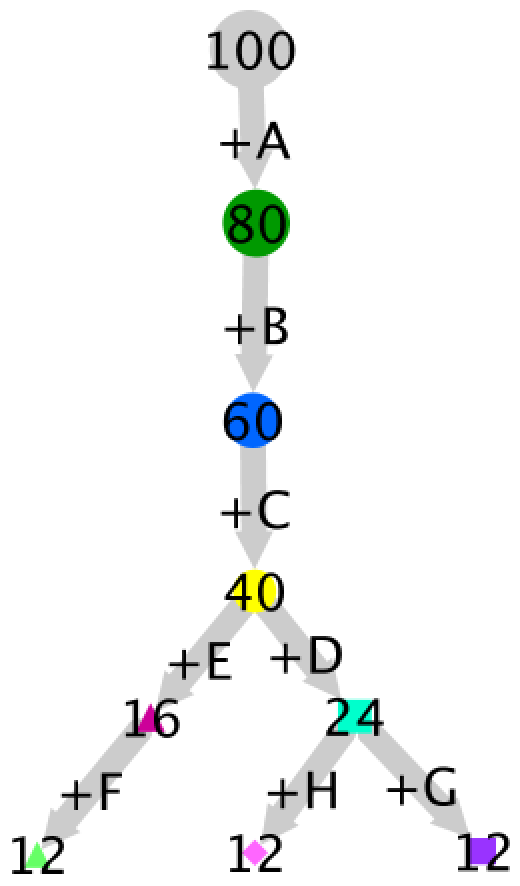
\includegraphics[width = 1.0\linewidth, trim={0 0 0 0}, clip=true]{graph1.png}
		\caption{}
		\label{1}
	\end{subfigure}
	\hspace{0.07\linewidth}
	\begin{subfigure}[t]{0.0452\linewidth}
		\centering
		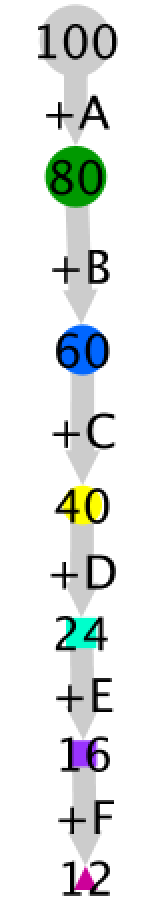
\includegraphics[width = 1.0\linewidth, trim={0 0 0 0}, clip=true]{graph2.png}
		\caption{}
		\label{2}
	\end{subfigure}
	\hspace{0.07\linewidth}
	\begin{subfigure}[t]{0.11\linewidth}
		\centering
		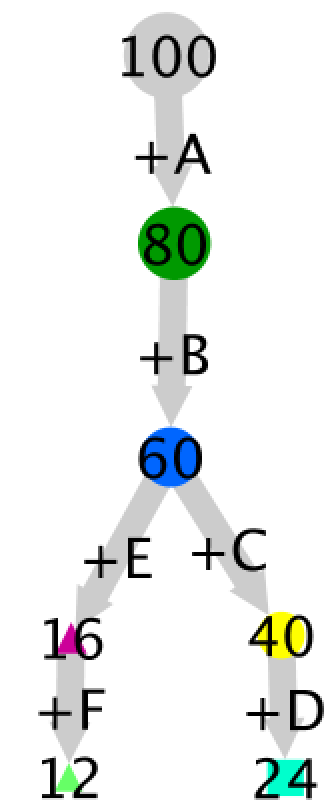
\includegraphics[width = 1.0\linewidth, trim={0 0 0 0}, clip=true]{graph3.png}
		\caption{}
		\label{3}
	\end{subfigure}
\caption{\textbf{(a)} example of summary bulk sequencing data given mutation count for different cellular frequencies. In reality, data is noisy and this noise-free diagram must be inferred by clustering. \textbf{(b)-(d)} examples of clonal phylogeny consistent with the data in (a). Labels on nodes indicate cellular frequencies for the most recently acquired mutation.}
\end{figure}


If we also want to infer copy numbers using bulk sequencing data, we can use the full per-locus read count ratios $D_j$ and allelic read counts $R_{jB_j}$ to set up a Hidden Markov Model allowing us to infer maximum likelihood cancer cell fractions $\tau_j$ and copy numbers $(c_A, c_B)$ at all our loci of interest along the genome. In the case of single cell data, we can instead infer relative copy number data directly from the sequencing data, and convert this to absolute copy number using paired normal samples.


\section*{Appendix}

\lstinputlisting[language=python]{ce_a1.py}

\end{document}


\begin{figure}[h]
	\centering
	\begin{subfigure}[t]{0.40\linewidth}
		\centering
		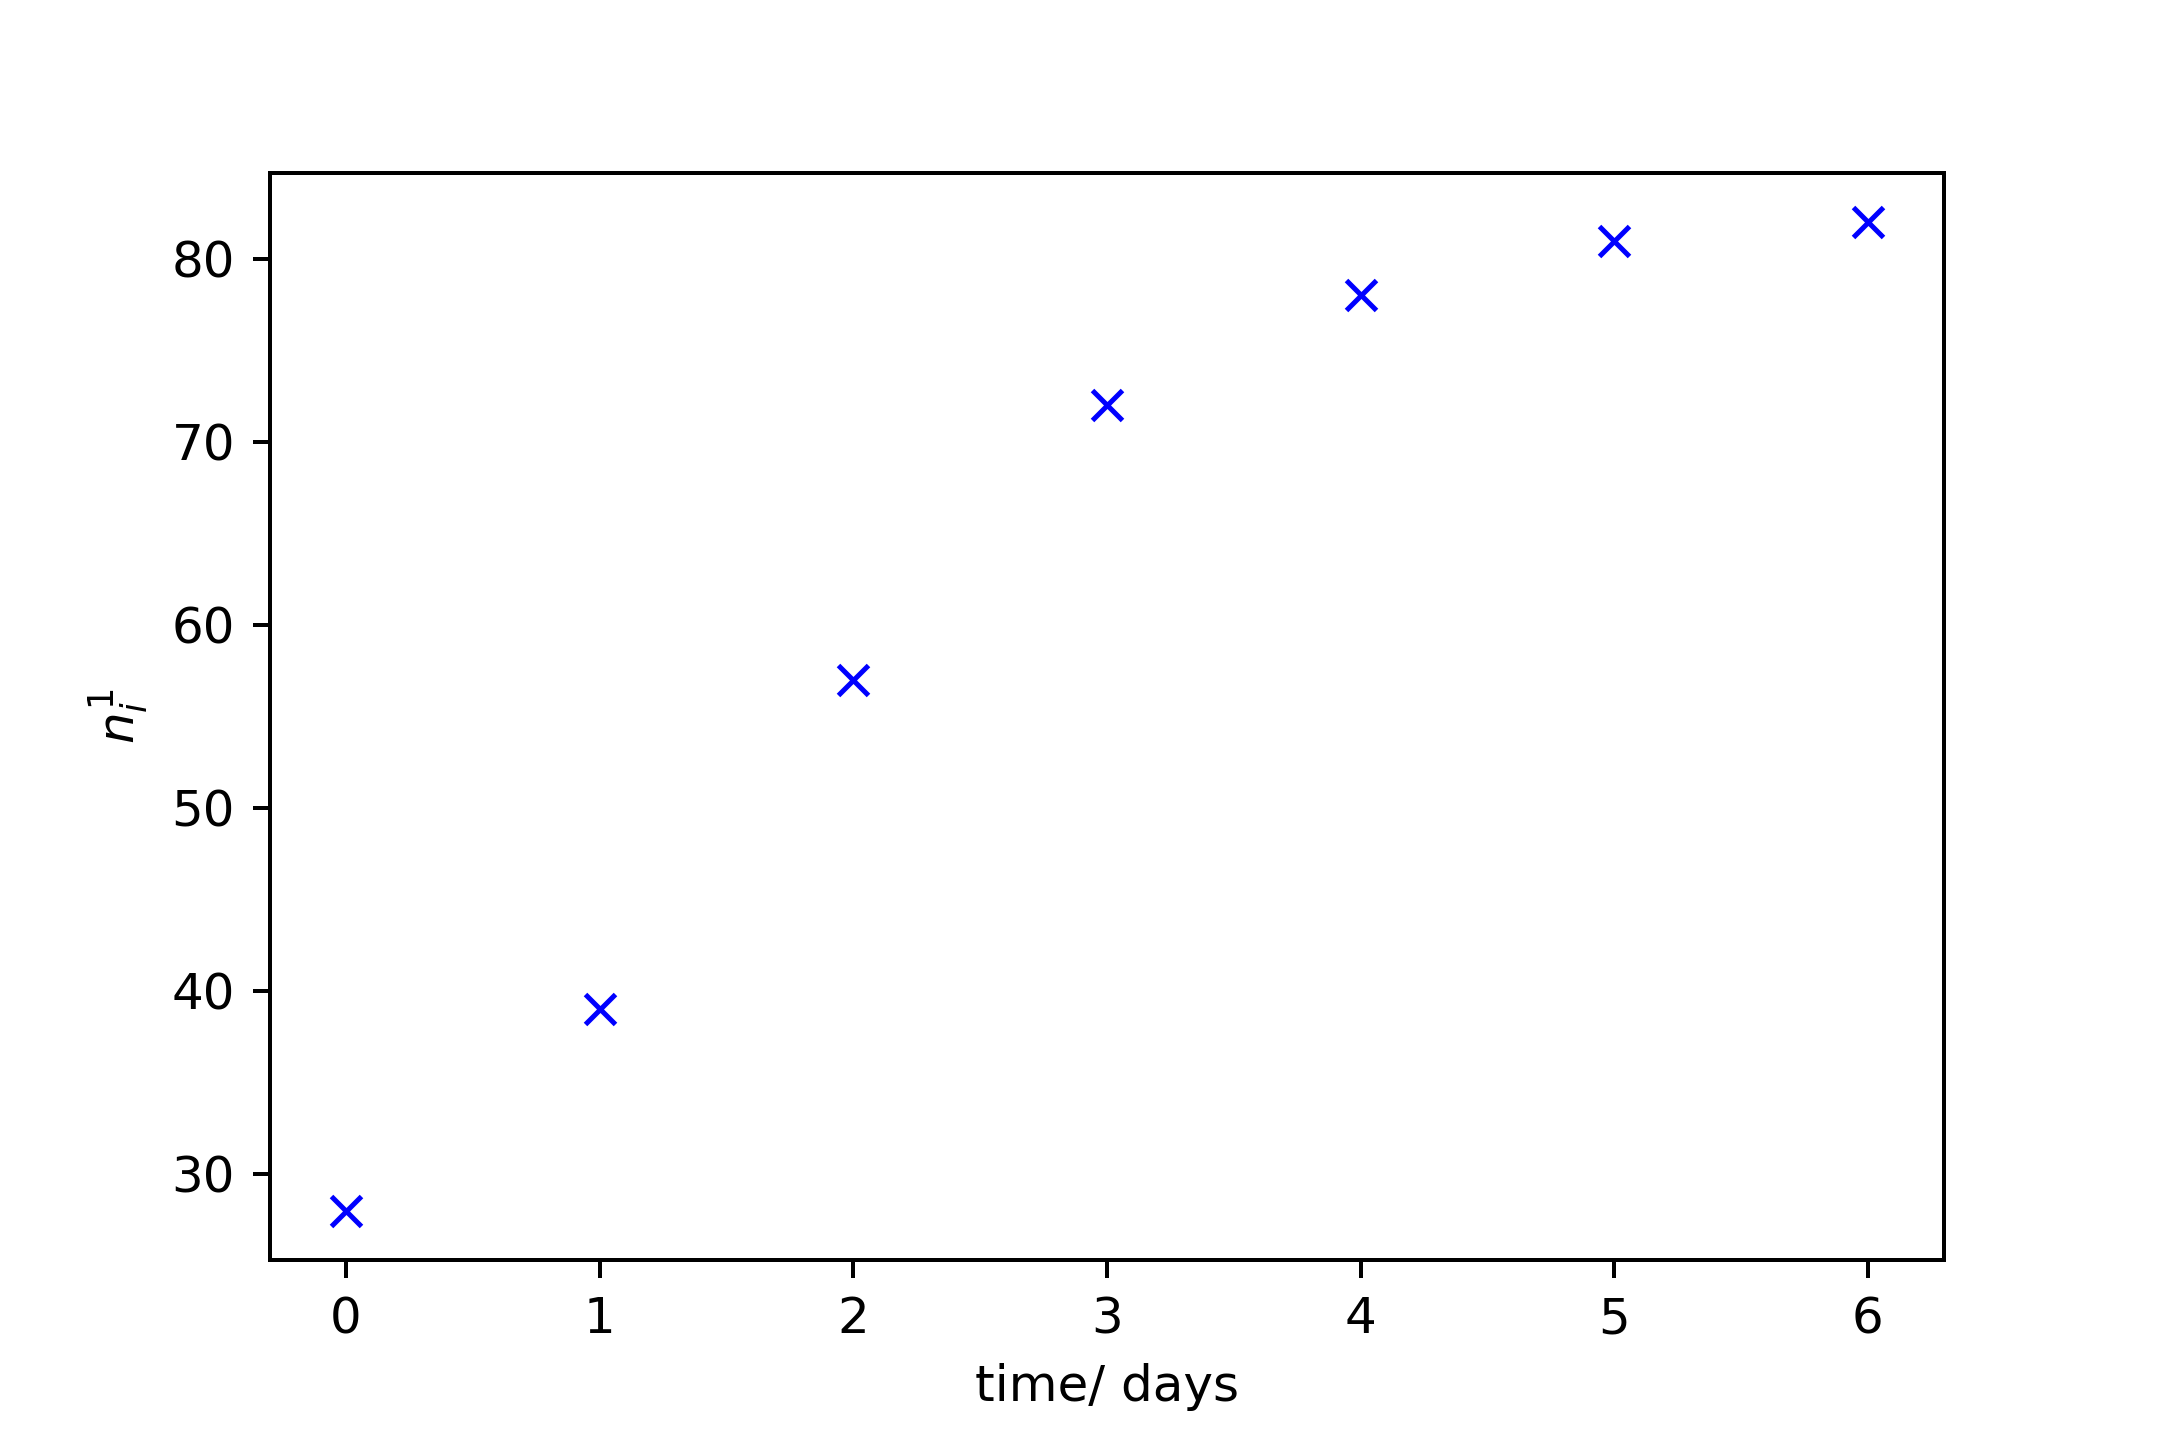
\includegraphics[width = 1.0\linewidth, trim={0 0 0 0}, clip=true]{data.png}
		\subcaption{$n_i^1$ at the 7 timepoints for which data is given.}
		\label{fig:data}	
	\end{subfigure}%
	\hspace{0.05\linewidth}
	\begin{subfigure}[t]{0.50\linewidth}
		\centering
		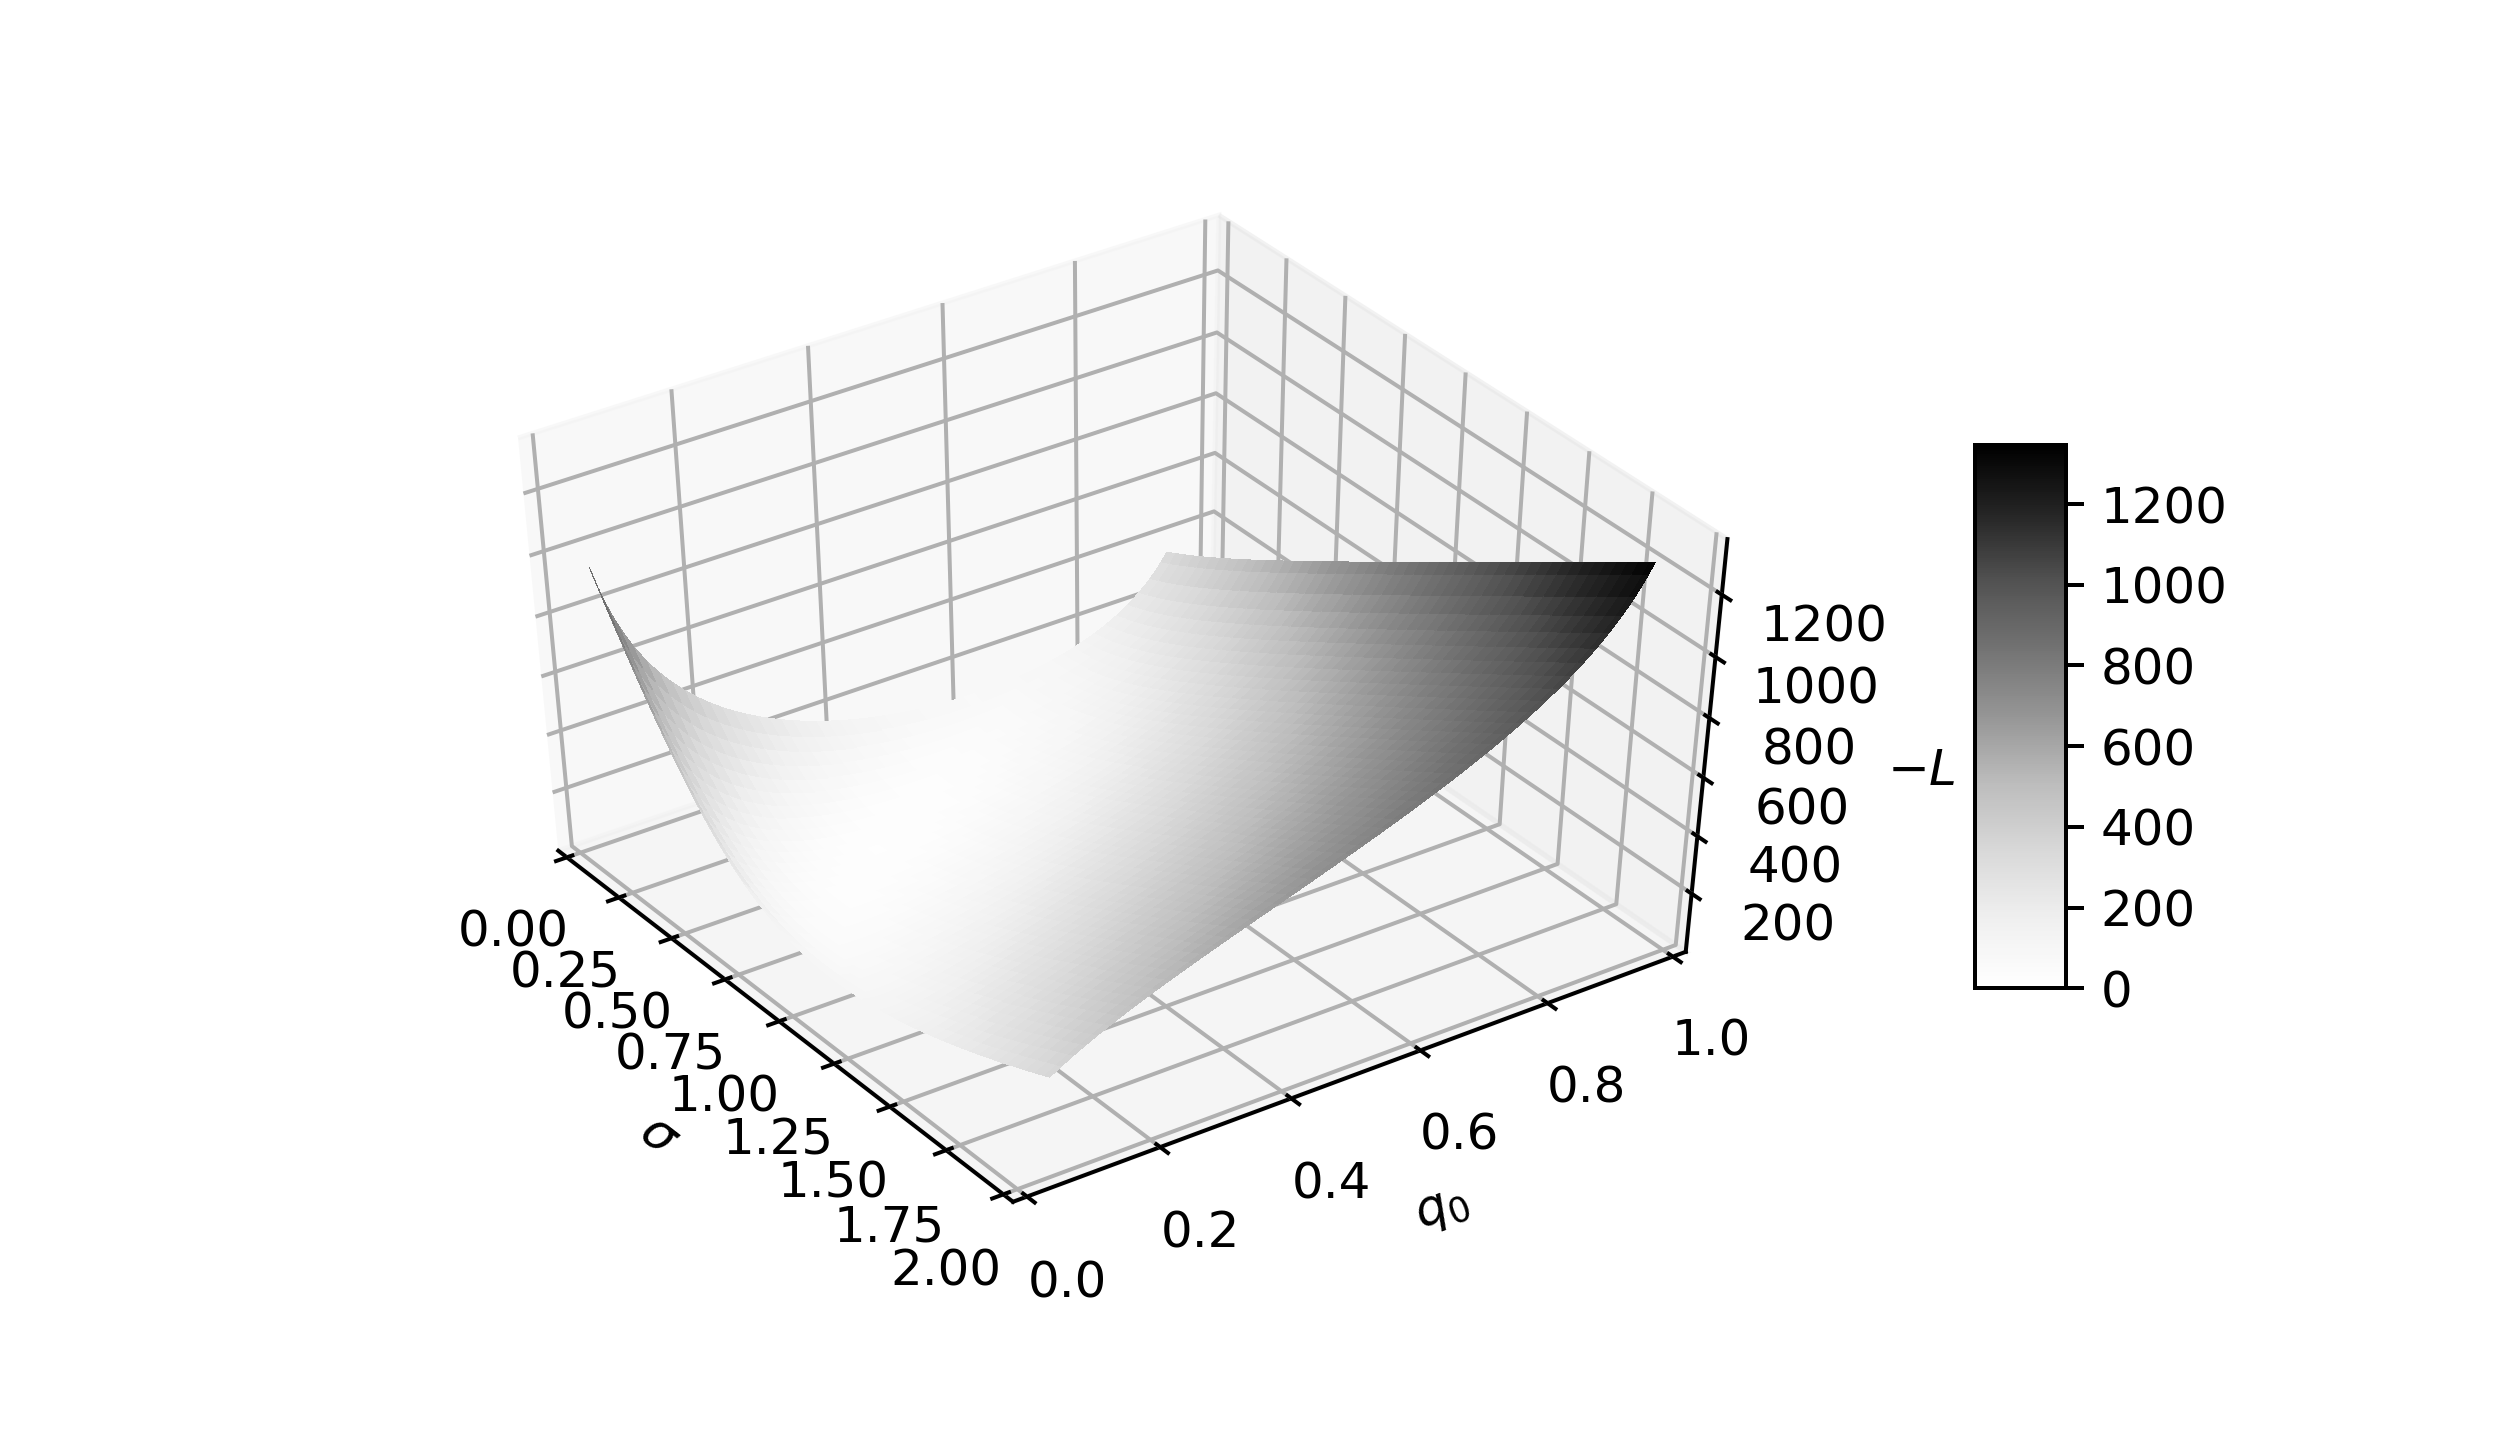
\includegraphics[width = 1.0\linewidth, trim={80 30 50 50}, clip=true]{Lsurf.png}
		\caption{Log likelihood of the observed data given different combinations of model parameters.}
		\label{fig:Lsurf}
	\end{subfigure}
\end{figure}



\begin{figure}[h]
	\centering
	\begin{subfigure}[t]{0.40\linewidth}
		\centering
		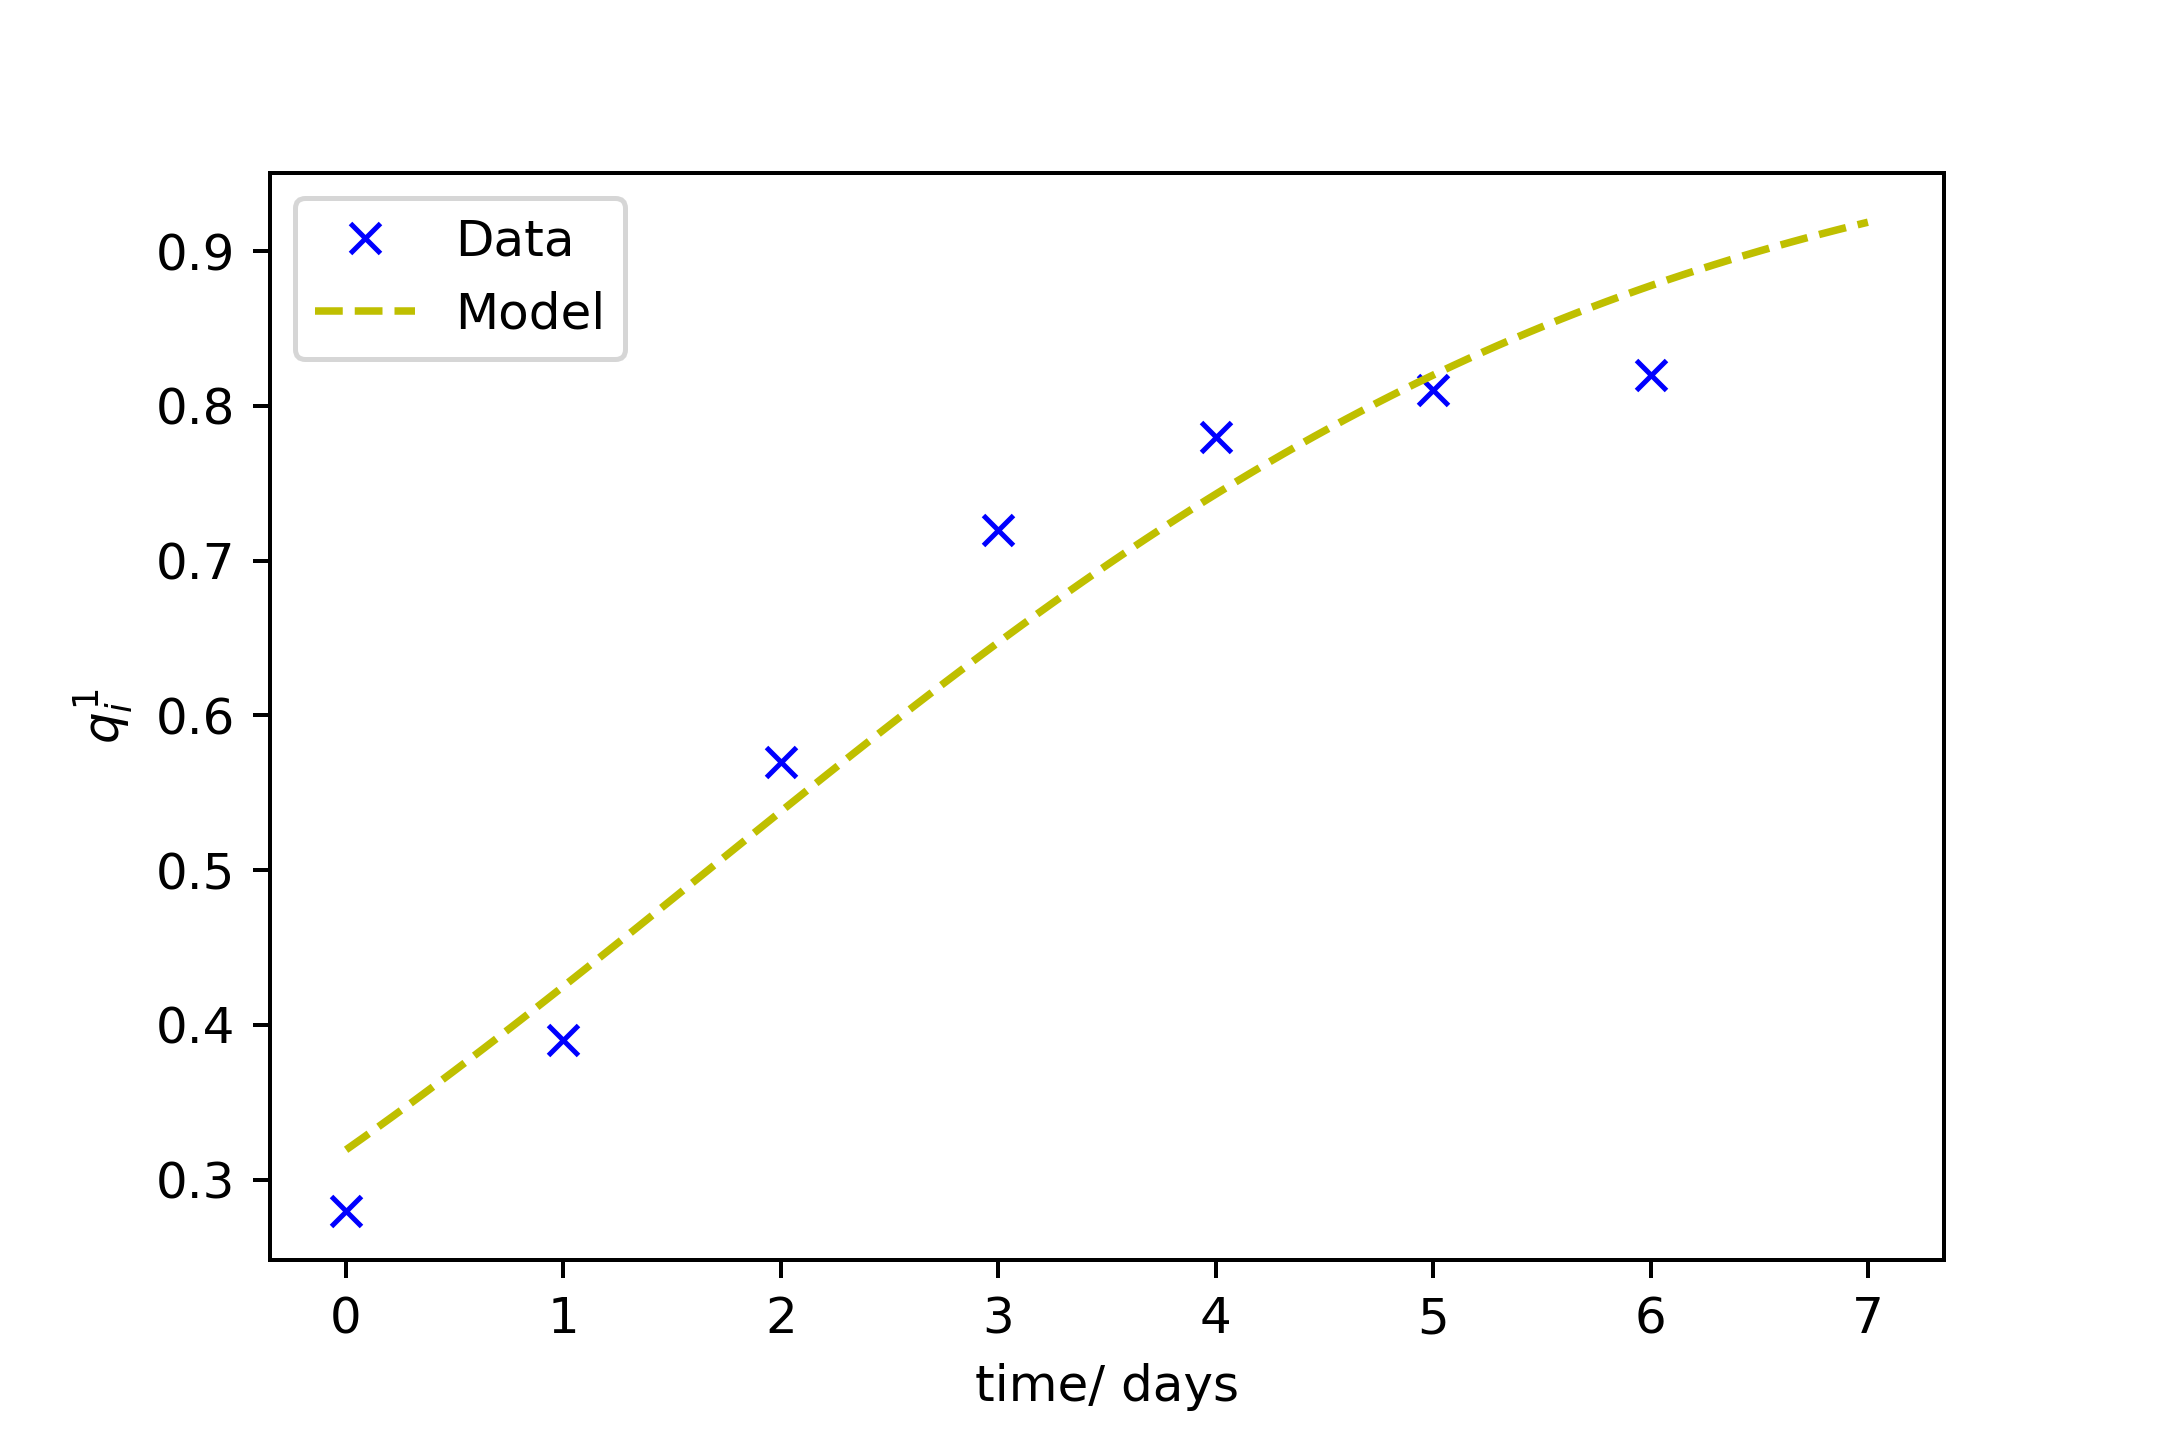
\includegraphics[width = 1.0\linewidth, trim={0 0 0 0}, clip=true]{fit_model.png}
		\subcaption{$q_i^1$ of 100 samples at the 7 timepoints for which data is given, and $q_i^1$ versus time as predicted by the MLE model.}
		\label{fig:fitted}	
	\end{subfigure}%
	\hspace{0.05\linewidth}
	\begin{subfigure}[t]{0.50\linewidth}
		\centering
		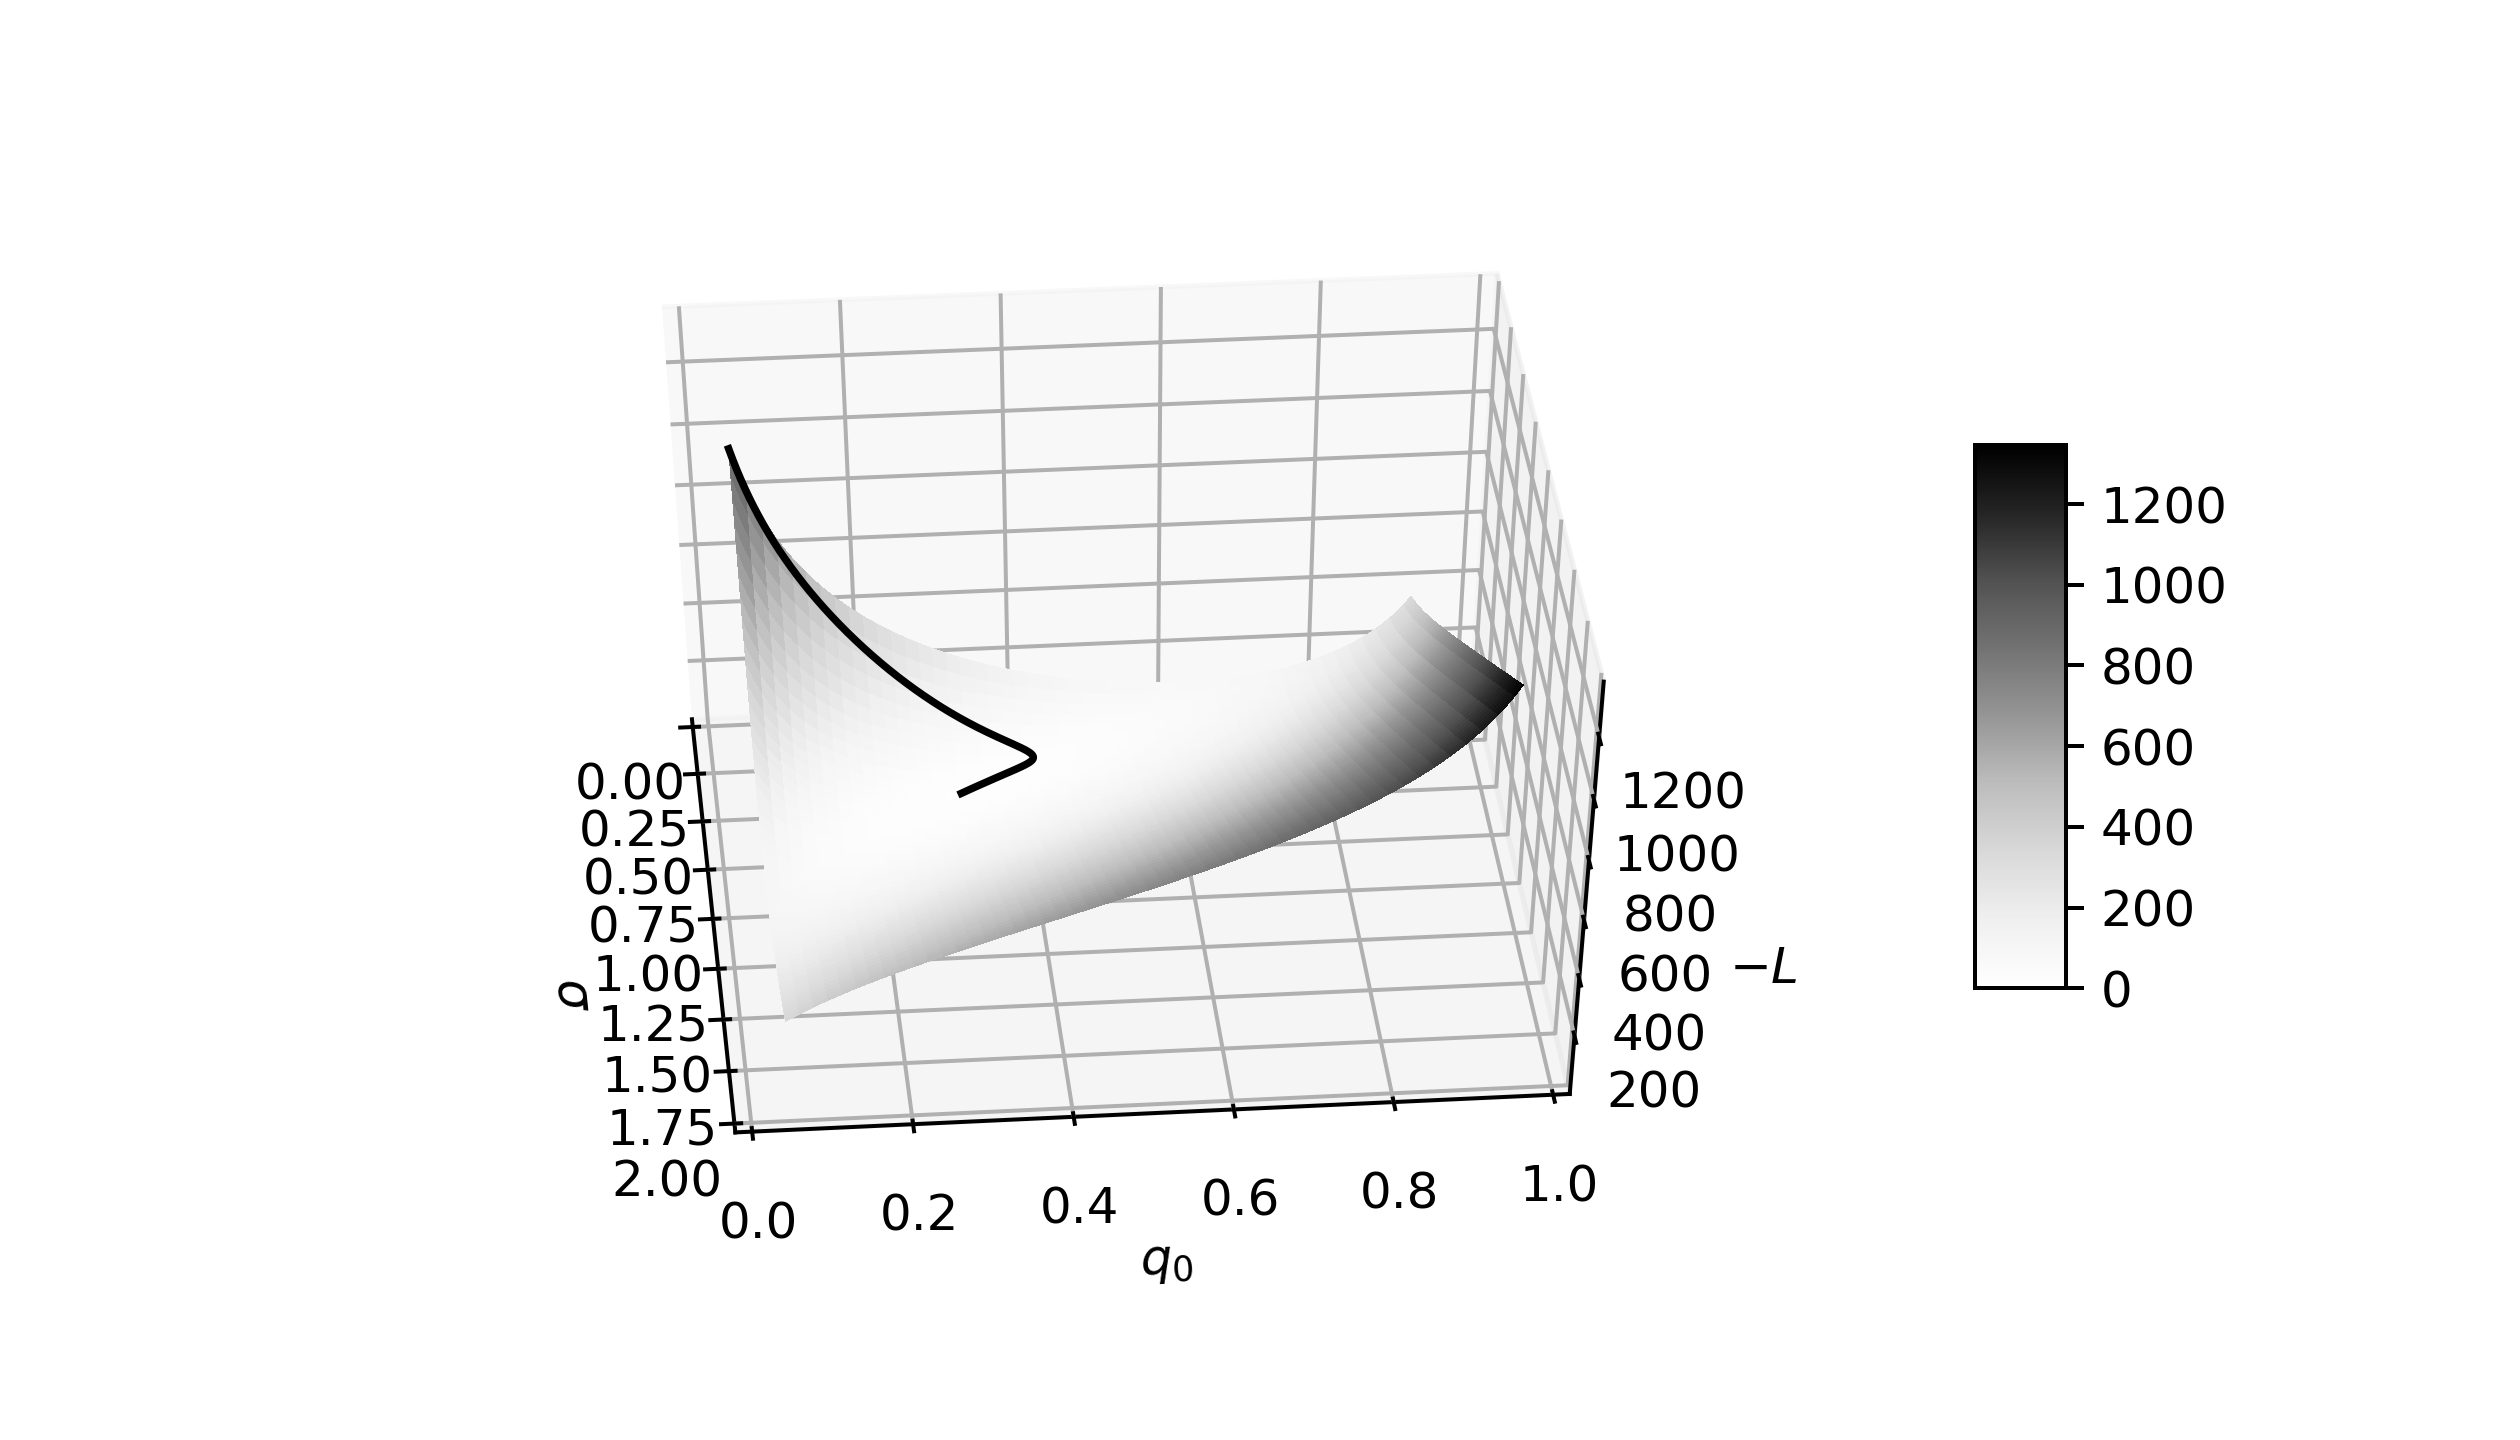
\includegraphics[width = 1.0\linewidth, trim={90 40 60 60}, clip=true]{Lsurfproj.png}
		\caption{Log likelihood of the observed data given different combinations of model parameters. Superimposed on this surface is the steepest descent path for parameter optimization. The same minimum was converged to with a range of different initial parameters.}
		\label{fig:Lsurfdesc}
	\end{subfigure}
\end{figure}